\documentclass[conference]{IEEEtran}
\usepackage[top=3cm, bottom=2cm, left=2cm, right=2cm, columnsep=20pt]{geometry}
\usepackage{pdfpages}
\usepackage{graphicx}
\usepackage{etoolbox}
\apptocmd{\sloppy}{\hbadness 10000\relax}{}{}
% \usepackage[numbers]{natbib}
\usepackage[T1]{fontenc}
\usepackage{ragged2e}
\usepackage[french]{babel}
\usepackage{listings}
\usepackage{color}
\usepackage{soul}
\usepackage[utf8]{inputenc}
\usepackage[export]{adjustbox}
\usepackage{caption}
\usepackage{mathrsfs, amsmath}
\usepackage{amssymb}
\usepackage{float}
\usepackage{csquotes}
\usepackage{fancyhdr}
\usepackage{wallpaper}
\usepackage{siunitx}
\usepackage[indent]{parskip}
\usepackage{textcomp}
\usepackage{gensymb}
\usepackage{multirow}
\usepackage[hidelinks]{hyperref}
\usepackage{abstract}
\usepackage{subcaption}
\usepackage{tabularx}
\usepackage{biblatex}
\addbibresource{bibliographie.bib}
% \renewcommand{\abstractnamefont}{\normalfont\bfseries}
% \renewcommand{\abstracttextfont}{\normalfont\itshape}
\usepackage{titlesec}
% \titleformat{\section}{\large\bfseries}{\thesection}{1em}{}
% \titleformat{\subsection}{\normalsize\bfseries}{\thesubsection}{1em}{}
% \titleformat{\subsubsection}{\normalsize\bfseries}{\thesubsubsection}{1em}{}

\usepackage{xcolor}
\definecolor{codegreen}{rgb}{0,0.6,0}
\definecolor{codegray}{rgb}{0.5,0.5,0.5}
\definecolor{codepurple}{rgb}{0.58,0,0.82}
\definecolor{backcolour}{rgb}{0.95,0.95,0.92}
\lstdefinestyle{mystyle}{
    backgroundcolor=\color{backcolour},   
    commentstyle=\color{codegreen},
    keywordstyle=\color{magenta},
    numberstyle=\tiny\color{codegray},
    stringstyle=\color{codepurple},
    basicstyle=\ttfamily\footnotesize,
    breakatwhitespace=false,         
    breaklines=true,                 
    captionpos=b,                    
    keepspaces=true,                 
    numbers=left,                    
    numbersep=5pt,                  
    showspaces=false,                
    showstringspaces=false,
    showtabs=false,                  
    tabsize=2
}
\lstset{style=mystyle}

\usepackage[most]{tcolorbox}
\newtcolorbox{note}[1][]{
  enhanced jigsaw,
  borderline west={2pt}{0pt}{black},
  sharp corners,
  boxrule=0pt, 
  fonttitle={\large\bfseries},
  coltitle={black},
  title={Note:\ },
  attach title to upper,
  #1
}


%----------------------------------------------------

\setlength{\parindent}{0pt}
\DeclareCaptionLabelFormat{mycaptionlabel}{#1 #2}
\captionsetup[figure]{labelsep=colon}
\captionsetup{labelformat=mycaptionlabel}
\captionsetup[figure]{name={Figure }}
\captionsetup[table]{name=Tableau}
\newcolumntype{Y}[1]{>{\Centering\hspace{0pt}\hsize=#1\hsize}X}
\newcommand{\inlinecode}{\normalfont\texttt}
\usepackage{enumitem}
\setlist[itemize]{label=\textbullet}

\begin{document}

%----------------------------------------------------
\title{Spectromètre\\
\large Travail préparatoire \\
PHS3910 -- Techniques expérimentales et instrumentation\\ 
Équipe L3}

\author{\IEEEauthorblockN{Émile Guertin-Picard}
\IEEEauthorblockA{2208363}
\and
\IEEEauthorblockN{Maxime Rouillon}
\IEEEauthorblockA{2213291}
\and
\IEEEauthorblockN{Marie-Lou Dessureault}
\IEEEauthorblockA{2211129}
\and
\IEEEauthorblockN{Philippine Beaubois}
\IEEEauthorblockA{2211153}
}

\maketitle

\textit{\textbf{Résumé} -- yap yap}

\section{Introduction}
yap yap

\section{Méthodes \label{methodes}}
Le système optique du spectromètre est schématisé dans la figure \ref{4f}.
\begin{figure}[H]
    \centering
    \includegraphics[scale=0.4]{4f.png}
    \caption{Schéma simplifié du spectromètre avec toutes ses composantes. \label{4f} \cite{procedurier}}
\end{figure}
Le parcours d'un faisceau passant à travers le spectromètre a été simulé à l'aide 
de l'optique de Fourier. Le champ initial a été modélisé par une fonction rectangle en deux dimensions,
afin de modéliser la forme du champ après avoir traversé une fente. Celui-ci peut donc être décrit par:
\[U(x_0,y_0)=rect(\frac{y_0}{b})rect(\frac{x_0}{a}),\]
où $a$ et $b$ sont la largeur et la hauteur de la fente respectivement. Le champ transmis par 
la première lentille a donc pu être déterminé:
\begin{align*}
    U_1(x_1,y_1)&\propto\mathscr{F}\left\{U(x_0,y_0)\right\}(\frac{x_1}{\lambda f_1},\frac{y_1}{\lambda f_1})\\
    &\propto \mathscr{F}\left\{rect(\frac{y_0}{b})rect(\frac{x_0}{a})\right\}(\frac{x_1}{\lambda f_1},\frac{y_1}{\lambda f_1})\\
    &\propto sinc(\frac{y_1b}{\lambda f_1})\ast sinc(\frac{x_1a}{\lambda f_1}),
\end{align*}
où $f_1$ est la longueur focale de la lentille. Le réseau de diffraction blazé modifie la forme du champ, ce qui a pu être
modélisé à l'aide d'un masque \cite{procedurier}:
\[M(x_1,y_1)=(comb(\frac{x_1}{\Lambda})\ast rect(\frac{x_1}{\Lambda})e^{i\beta x})rect(\frac{x_1}{N\Lambda}).\]
Ici, la forme du champ n'est pas limitée par la grandeur du réseau de diffraction, mais par les dimensions
de la fente; le terme $rect(x_1/N\Lambda)$ a pu être négligé. Le champ à la sortie de la deuxième lentille revient à effectuer la transformée de Fourier
de $U_1(x_1,y_1)$:
\begin{align*}
    U_2\propto&\ \mathscr{F}\left\{sinc(\frac{y_1b}{\lambda f_1})\ast sinc(\frac{x_1a}{\lambda f_1})M\right\}(\frac{x_2}{\lambda f_2},\frac{y_2}{\lambda f_2})\\
    \propto&\ rect(\frac{y_2 f_1}{b f_2})rect(\frac{x_2 f_1}{a f_2})\ast comb(\frac{x_2 \Lambda}{\lambda f_2})\\
    &\ sinc(\frac{x_2 \Lambda}{\lambda f_2})\ast \delta(2\pi(x_2-\frac{\beta}{2\pi}))\\
    \propto&\ rect(\frac{y_2 f_1}{b f_2})rect(\frac{x_2 f_1}{a f_2})\ast comb(\frac{x_2 \Lambda}{\lambda f_2})\\
    &\ sinc(\frac{\Lambda}{\lambda f_2}(x_2-\frac{\lambda f_2 \beta}{2\pi})).
\end{align*}
Pour évaluer le terme $rect(\frac{x_2 f_1}{a f_2})\ast comb(\frac{x_2 \Lambda}{\lambda f_2})$, la fonction $comb$ a été remplacée par sa définition:
\begin{align*}
    rect(\frac{x_2 f_1}{a f_2})\ast comb(\frac{x_2 \Lambda}{\lambda f_2})&=rect(\frac{y_2 f_1}{b f_2})\ast\sum_{\infty}\delta(x_2-\frac{n\lambda f_2}{\Lambda})\\
    &=\sum_{\infty}rect(\frac{f_1}{a f_2}(x_2-\frac{n\lambda f_2}{\Lambda})).
\end{align*}
En rassemblant tous les termes, on a obtenu:
\begin{align*}
    U_2(x_2,y_2)\propto&\ rect(\frac{y_2 f_1}{b f_2})\sum_{\infty}rect(\frac{f_1}{a f_2}(x_2-\frac{n\lambda f_2}{\Lambda}))\\
    & \ sinc(\frac{\Lambda}{\lambda f_2}(x_2-\frac{\lambda f_2 \beta}{2\pi})).
\end{align*}
On sait que $\beta x = \phi$, où $\phi$ est le décalage de phase entre deux faisceaux à la sortie du réseau de diffraction.
La différence de parcours $\delta(x)$ est directement reliée au décalage de phase par $\phi=2\pi\delta(x)/\lambda$, où $\delta(x)=2tan\theta x$.
Ce résultat est illustré dans la figure \ref{beta}. 
\begin{figure}[H]
    \centering
    \includegraphics[scale=0.2]{beta.png}
    \caption{Représentation de la différence de parcours de deux faisceaux sur un réseau de diffraction
    blazé. Ici, $\lambda_B$ correspond à la longueur d'onde de Blaze. \label{beta}}
\end{figure}
En faisant l'approximation des petits angles $tan\theta\approx\theta$, on retrouve:
\begin{align*}
   \beta x &=\frac{2\pi\delta(x)}{\lambda} \approx\frac{4\pi\theta x}{\lambda}\\
   \beta&\approx \frac{4\pi\theta}{\lambda}
\end{align*} 
Avec l'équation de Bragg pour la diffraction, et en choisissant l'ordre $m=1$, on a trouvé que $2\Lambda sin\theta=\lambda_B \rightarrow \theta\approx\lambda_B/2\Lambda$.
On a donc:
\begin{align*}
   \beta&\approx \frac{2\pi\lambda_B}{\lambda\Lambda}.
\end{align*}
En remplaçant ce terme dans la fonction $sinc$, on a $sinc(\frac{\Lambda}{\lambda f_2}(x_2-\frac{\lambda_B f_2}{\Lambda}))$. En comparant cette
fonction $sinc$ avec la fonction $rect$ en $x$, on a pu remarquer que le terme $n=1$ de la somme s'aligne parfaitement 
avec la fonction $sinc$ lorsque $\lambda=\lambda_B$, où $\lambda_B$ est la longueur d'onde de Blaze. Par conséquent, on considère que pour des longueurs d'onde proches
de $\lambda_B$, l'ordre $n=1$ est aussi suffisament aligné à la fonction $sinc$. La forme de $sinc$ nous a permis d'éliminer tous les autres termes $n\neq1$, et on a obtenu:
\begin{align*}
    U_2(x_2,y_2)\propto&\ rect(\frac{y_2 f_1}{b f_2})rect(\frac{f_1}{a f_2}(x_2-\frac{\lambda f_2}{\Lambda}))\\
    & \ sinc(\frac{\Lambda}{\lambda f_2}(x_2-\frac{\lambda f_2}{\Lambda})).
\end{align*}
Les largeurs du $sinc$ et du $rect$ en $x$ sont proportionnelles à $\lambda f_2/\Lambda$ et $af_2/f_1$, respectivement, ce qui nous
a permis de traiter $sinc\approx1$ parce que l'ordre de grandeur (pour les contraintes du projet) de $\lambda/\Lambda$ est de $\approx10^{-1}$ alors que celui de $a/f_1$ est
de $\approx10^{-2}$. La forme finale de $U_2(x_2,y_2)$ est:
\begin{align*}
    U_2(x_2,y_2)\propto&\ rect(\frac{y_2 f_1}{b f_2})rect(\frac{f_1}{a f_2}(x_2-\frac{\lambda f_2}{\Lambda})).
\end{align*}
Une contrainte du projet consiste à ce que la largeur du spectre d'ordre 1 capté par la caméra
soit d'une largeur équivalente ou légèrement inférieure à la largeur de la caméra. Mathématiquement, ceci correspond à
$x(\lambda_{bleu})-x(\lambda_{rouge})\leq D_{cam}$. On a pu approximer que $x(\lambda)$ correspond au terme de décalage
de la fonction $rect$ en $x$. Les dimensions de la caméra utilisée pour le spectromètre sont de 1280 x 1024 pixels, chacun étant un carré de
$5.2\ \mu m$ côté. La zone sensible de la caméra est donc de 6.656 x 5.323 mm \cite{camera}. Par conséquent, il a été nécessaire d'optimiser la relation suivante
en fonction des lentilles disponibles (25, 30, 50 ou 100 mm de longueur focale):
\begin{align*}
    \frac{f_2}{\Lambda}(\lambda_{bleu}-\lambda_{rouge})\leq 6.656\ mm.
\end{align*}
Ayant une valeur de $f_2$ déterminée, la résolution du spectromètre a pu ensuite être optimisée. La résolution a été trouvée en
considérant que deux longueurs d'onde voisines, $\lambda_1$ et $\lambda_2$, se touchent à une valeur de $x$ qui correspond à:
\begin{align*}
    x=\frac{a f_2}{2f_1}+\frac{\lambda_1 f_2}{\Lambda}&=-\frac{a f_2}{2f_1}+\frac{\lambda_2 f_2}{\Lambda}\\
    \frac{af_2}{f_1}&=\frac{f_2}{\Lambda}(\lambda_2-\lambda_1)\\
    \delta_{\lambda}&=\lambda_2-\lambda_1=\frac{\Lambda a}{f_1}
\end{align*}
\section{Résultats \label{resultats}}
En considérant $\lambda_{bleu}=380\ nm$ et $\lambda_{rouge}=780\ nm$, les largeurs des spectres obtenues sont présentées
dans le tableau \ref{largeur_spectre}.
\begin{table}[H]
    \caption{Résultats des largeurs de spectres pour des lentilles ayant des longueurs focales
    $f_2$ de 10, 15, 20, 25, 30, 50 ou 100 mm. Le réseau de diffraction a 600 lignes/mm, ce qui correspond à un pas de réseau
    de $\Lambda=1/600$ mm \cite{grating}.}    
    \centering
    \begin{tabular}{c|c|c|c}
    $\Lambda$ (mm) & $f_2$ (mm) & $D_{spectre}$ (mm) & $\Delta_D$ \\
    \hline
    \hline
    \multirow{7}{*}{1/600} & 10 & 2.40 & -4.256 \\
    & 15 & 3.60 & -3.056 \\
    & 20 & 4.80 & -1.856 \\
    & 25 & 6 & -0.656 \\
    & 30 & 7.20 & 0.544 \\
    & 50 & 12 & 5.344 \\
    & 100 & 24 & 17.344\\
    \hline
    \end{tabular}
    \label{largeur_spectre}
\end{table}
La résolution a été déterminée pour des valeurs de $a$ allant de 0 à 3 mm et pour les lentilles
disponibles. Les résultats sont présentés dans la figure \ref{res}.
\begin{figure}[H]
    \centering
    \includegraphics[scale=0.5]{Resolution.png}
    \caption{Résolution du spectromètre en fonction de la largeur de la fente $a$ et la longueur focale $f_1$
    de la lentille \label{res}}
\end{figure}

\section{Discussion}
Tel que démontré mathématiquement dans la section \ref{methodes}, l'ordre $n=1$ est optimal pour visualiser la diffraction
du faisceau entrant. Physiquement, l'ordre $n=0$ n'est pas pertinent pour le contexte d'un spectromètre parce qu'il ne présente que 
la réflection du faisceau. La diffraction est seulement visible pour les ordres $|n|\leq0$, et ce, avec beaucoup plus d'intensité pour l'ordre $n=1$.
Par conséquent, l'axe optique à la sortie du réseau de diffraction doit être alignée avec l'ordre $n=1$ et non l'ordre $n=0$, ce qui impose
de positionner le réseau de diffraction à un angle particulier. \textcolor{red}{explication de l'angle d'incidence et de sortie}.

En évaluant les résultats des longueurs focales $f_2$ et en considérant la condition initiale
$x(\lambda_{bleu})-x(\lambda_{rouge})\leq 6.656$ mm, les seules lentilles acceptables sont celles
ayant une longueur focale inférieure ou égale à 25 mm. En raison des dimensions physiques des composantes et de
la position du capteur de la caméra, les lentilles ayant des longueurs focales inférieures à 25 mm ne peuvent pas être utilisées.
Ceci élimine donc toutes les lentilles sauf celle de $f_2=25$ mm, ce qui limite le choix à celle-ci.

Pour ce qui est du choix de la longueur focale de la première lentille $f_1$, la relation inversement proportionnelle
entre la résolution et $f_1$ ($\Lambda a/f_1$) permet de déterminer qu'une longueur focale plus grande serait optimale. Cependant,
les limites imposées par l'impression 3D élimine le choix de $f_1=100$ mm. Une longueur focale $f_1$ de 50 mm est donc choisie.


\section{Annexes}

\subsection{Développement mathématique détaillé}
yap yap


\clearpage

\printbibliography
% \bibliographystyle{unsrtnat}
% \bibliography{My_Library}

\end{document}
